\documentclass[handout,11pt]{beamer}
\usetheme{Frankfurt}
%\usefonttheme{professionalfonts}


\usepackage[utf8]{inputenc}
\usepackage{physics}
\usepackage{graphicx}
\usepackage{tikz}
\usepackage{siunitx}

\author{Haikal Isa Al Mahdi}
\title{Analisis Dimensi}
%\setbeamercovered{transparent} 
%\setbeamertemplate{navigation symbols}{} 
%\logo{} 
%\institute{} 
%\date{} 
%\subject{} 
\begin{document}

\begin{frame}
\titlepage
\end{frame}

\begin{frame}
\tableofcontents
\end{frame}


\section{Pendahuluan}
\label{sec:Pendahuluan}

\begin{frame}{Kenapa?}

\begin{itemize}
\item Soal yang terkait dengan fisika (khususnya mekanika) dalam tingkat olimpiade tidak cukup diselesaikan hanya dengan menghafal rumus.
\item Kita tahu bahwa $F=ma$, namun situasi akan semakin rumit bila sistem semakin kompleks
\item Oleh karena itu, dalam hal ini diperlukan kemampuan problem-solving (setidaknya yang mendasar)
\end{itemize}
\end{frame}

\begin{frame}{Materi Prasyarat}
\begin{itemize}
\item Aljabar Dasar
\item Eksponen, Akar, dan Logaritma
\item Vektor
\item Kalkulus dasar (integral dan turunan)

\end{itemize}

Manipulasi aljabar terkadang sudah cukup untuk menyelesaikan soal.
\end{frame}


\begin{frame}{Dua Cara}
Berdasarkan metodenya, terdapat 2 jenis fisika:
\begin{enumerate}
  \item Fisika Aljabar
  \item Fisika Kalkulus
\end{enumerate}
Walaupun kita terbiasa menyelesaikan masalah fisika dengan fisika aljabar, tidak ada salahnya untuk mempelajari fisika kalkulus.

\end{frame}

\section{Metode Matematika}
\label{sec:Metode Matematika}

\begin{frame}[shrink]{Trigonometri}
  Fungsi trigonometri adalah perbandingan antara sisi-sisi segitiga.
  \begin{columns}[c]
  
  \column{0.5\textwidth}
  \begin{figure}[h]
  \begin{center}
  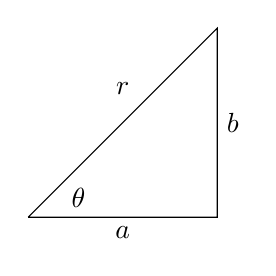
\begin{tikzpicture}[scale=0.8]
    \draw (0,0)--(3,0)--(3,3)--(0,0);
    \node[below] at (1.5,0) {$a$};
    \node[right] at (3,1.5) {$b$};
    \node[above] at (1.5,1.8) {$r$};
    
    \node[above] at (0.8,0) {$\theta$};
    
  \end{tikzpicture}
  \end{center}
  \caption{Segitiga Siku-Siku}
  \end{figure}
  
  
  \column{0.5\textwidth}
  \begin{block}{Fungsi}
    \begin{itemize}
      \item $\sin \theta = \frac{b}{r}$
      \item $\cos \theta = \frac{a}{r}$
      \item $\tan \theta = \frac{b}{a} = \frac{\sin \theta}{\cos \theta}$
    \end{itemize}
    Konsekuensinya,
    \begin{itemize}
      \item $r\sin \theta = b$
      \item $r\cos \theta = a$
    \end{itemize}
    Terdapat pula fungsi arcus (invers dari fungsi trigonometri)
    \begin{itemize}
      \item $\arcsin(\frac{b}{r}) = \theta$
      \item $\arccos(\frac{a}{r}) = \theta$
      \item $\arctan(\frac{b}{a}) = \theta$
    \end{itemize}
  \end{block}
  \end{columns}
\end{frame}

\begin{frame}{Skala}
  Terkadang kita menemukan pernyataan seperti
  "a berbanding lurus terhadap b".\\
  
 Apa artinya?
 \begin{itemize}
   \item $a \propto b$ artinya adalah "a berbanding lurus terhadap b"
   \item Perlu diketahui bahwa $a\propto b$ tidak sama dengan $a=b$
   \item Secara matematis, $a\propto b$ dapat dinyatakan sebagai $a = kb$ untuk suatu konstanta $k$
   \item Misalnya saja, luas lingkaran adalah $L = \pi r^2$. Dalam hal ini, $L \propto r^2$. Saat $r$ menjadi 2 kali lipat, Luasnya akan bertambah 4 kali lipat
   \item Jika diketahui $a_1 \propto \alpha_1$ dan $a_2 \propto \alpha_2$ (konstanta sama), maka
   $$\frac{a_1}{a_2} = \frac{\alpha_1}{\alpha_2}$$
  
 \end{itemize}
\end{frame}

\section{Analisis Dimensi}
\label{sec:Analisis Dimensi}

\begin{frame}{Analisis Dimensi}
  Analisis dimensi berguna dalam menentukan... dimensi dari suatu besaran.
  \begin{itemize}
    \item Amat erat kaitannya dengan eksponen
    \item Sering muncul pernyataan-pernyataan seperti "berbanding lurus", "berbanding terbalik", atau "bergantung pada" di dalam soal.
    \item Analisis dimensi dapat diterapkan pada metode integrasi.
    \item Cenderung mudah
  \end{itemize}
\end{frame}

\section{Contoh Soal}
\label{sec:Contoh Soal}

\begin{frame}{Contoh Soal dan Solusi}
Perkirakan rumus gaya hambat udara yang bergantung pada massa jenis udara ($\rho$), kecepatan angin ($v$), dan luas penampang lintang $A$.\\~\\
    
    \textbf{Solusi. } Jika pernyataan di atas diubah ke bentuk proporsi, maka akan menjadi
    $$F \propto \rho^x v^y A^z$$
    Kita tinjau dimensi dari masing-masing 
    \begin{itemize}
      \item $\rho = \unit{[M][L]^{-3}}$
      \item $v = \unit{[L][T]^{-1}}$
      \item $A = \unit{[L]^2}$
      \item $F = \unit{[M][L][T]^{-2}}$
    \end{itemize}
    dengan ini,
    $$\unit{[M][L][T]^{-2}} =\unit{[M]^x [L]^{-3x+y+2z} [T]^{-y}}$$
  \end{frame}
  
  \begin{frame}{Contoh Soal dam Solusi}
    
    Dapat dilihat bahwa 
    \begin{itemize}
      \item $x=1$
      \item $-3x+y+2z=1$
      \item $-y=-2$
    \end{itemize}
    Solusi dari sistem di atas adalah $x=1$, $y=2$, dan $z=1$. Dengan ini
    $$\boxed{F\propto \rho v^2 A}$$
    Selesai
\end{frame}


\begin{frame}{Contoh Lainnya}
  Diketahui bahwa untuk $x>1$
  $$\int{\frac{1}{x^2-1}}\dd x = \frac{1}{2}\ln(\frac{x-1}{x+1})$$
  Tentukan
  $$\int{\frac{1}{(ax)^2-1}}\dd x$$
\end{frame}

\begin{frame}{Solusi}
  Misalkan $x$ memiliki satuan meter $m$. $\dd x$ pun demikian. Agar $(ax)^2$ menjadi tak berdimensi, anggap $a=m^{-1}$. 
  Dengan demikian,
  $$\int{\frac{1}{(ax)^2-1}}\dd x \propto m$$
  Pada titik ini, kita mesti mencari nilai $\phi$ sehingga $a^\phi = m$. mengingat $a=m^{-1}$, persamaannya menjadi
  $$m^{-\phi}=m$$
  Yang mana jawabannya adalah $\phi=-1$ sehingga 
  $$\int{\frac{1}{(ax)^2-1}}\dd x \propto \frac{1}{a}$$
\end{frame}

\begin{frame}{Solusi}
  Sekarang, secara kasarnya, kita dapatkan 
  $$\int{\frac{1}{(ax)^2-1}}\dd x = \frac{1}{2a}\ln(\frac{x-1}{x+1})$$
  Namun, argumen di dalam fungsi logaritma natural tersebut haruslah tak berdimensi. Artinya,
  $$\int{\frac{1}{(ax)^2-1}}\dd x = \frac{1}{2a}\ln(\frac{ax-1}{ax+1})$$
\end{frame}

\frame{
  \begin{block}{Catatan}
    Terdapat beberapa hal yang perlu diperhatikan ketika bermatematika dalam fisika
    \begin{itemize}
      \item Olimpiade fisika bukanlah ujian integral. Jika memang diharuskan memakai integral, biasanya terdapat petunjuk (hint) di dalam soal. (Petunjuk: $\int{\frac{1}{ax+b}\dd x} = \frac{1}{a}\ln(ax+b)$)
      \item Fungsi $\sin x, \cos x, \tan x, \log x, \exp(x)$ dan semisalnya \textbf{tidak berdimensi}
      \item Perhatikan arah vektornya
      \item Telitilah dalam pemroyeksian vektor ($r\sin \theta, r\cos \theta$)
    \end{itemize}
  \end{block}
  
  Bacaan lebih lanjut dapat dilihat di \url{knzhou.github.io/handouts/P1.pdf}
}

\end{document}